% ============================================================
% Section 5: Discussion and independent online-style validation
% Dependencies: \usepackage{graphicx,booktabs}
% Copy figure files to your manuscript's figures/ folder.
% ============================================================
\section{Discussion and online validation}
\label{sec:discussion_online}

\subsection{Independent verification on Weld 09}
\label{sec:w09_verification}

To further assess the applicability of PI-NGreyKAN beyond the four welding cases used in the comparative experiments, an independent cross-weld validation was performed using Weld 09 (W09). In this experiment, all 528 observations from Cases 1--4 were used to train the model, without reserving any of these observations as a final testing subset. The training duration was fixed at 15 epochs based on the earlier experiments on Cases 1--4, and three random seeds (2026, 2027, and 2028) were used. The thermal decay scale and penetration-depth loss weight were fixed at $\ell=0.5$ and $\alpha=0.6$, respectively. The resulting model parameters and data normalization statistics were fixed before W09 was processed.

W09 contains 193 chronologically ordered observations of welding current, voltage, tracking error, and sound pressure level, along with the measured penetration depth and weld width. During validation, only the four sensor inputs were supplied sequentially to the pretrained model, and the grey dynamic state was updated recursively without using any observed W09 outputs. The mean of the predictions from the three independently trained models was used to obtain the reported estimates. The measured W09 outputs were used exclusively for subsequent error assessment. This protocol simulates the inference stage of an online monitoring system, but does not constitute a deployment test on an operating welding controller.

The prediction results are shown in Fig.~\ref{fig:w09_online_prediction}, and their quantitative evaluation is summarized in Table~\ref{tab:w09_online_metrics}. PI-NGreyKAN achieves an MAE of 0.0478~mm, an RMSE of 0.1345~mm, and a MAPE of 0.8579\% for penetration depth. For weld width, the corresponding errors are 0.0995~mm, 0.1290~mm, and 2.5223\%, respectively. For descriptive assessment of prediction-error coverage, a relative-error tolerance of 5\% is used. Under this criterion, 185 of 193 penetration-depth predictions (95.9\%) and 165 of 193 weld-width predictions (85.5\%) fall within the specified tolerance. Both prediction targets satisfy the 5\% tolerance simultaneously at 158 observations, corresponding to 81.9\% of W09. These error-tolerance percentages are statistical measures of predictive agreement, rather than industrial weld acceptance rates.

\begin{figure}[htbp]
    \centering
    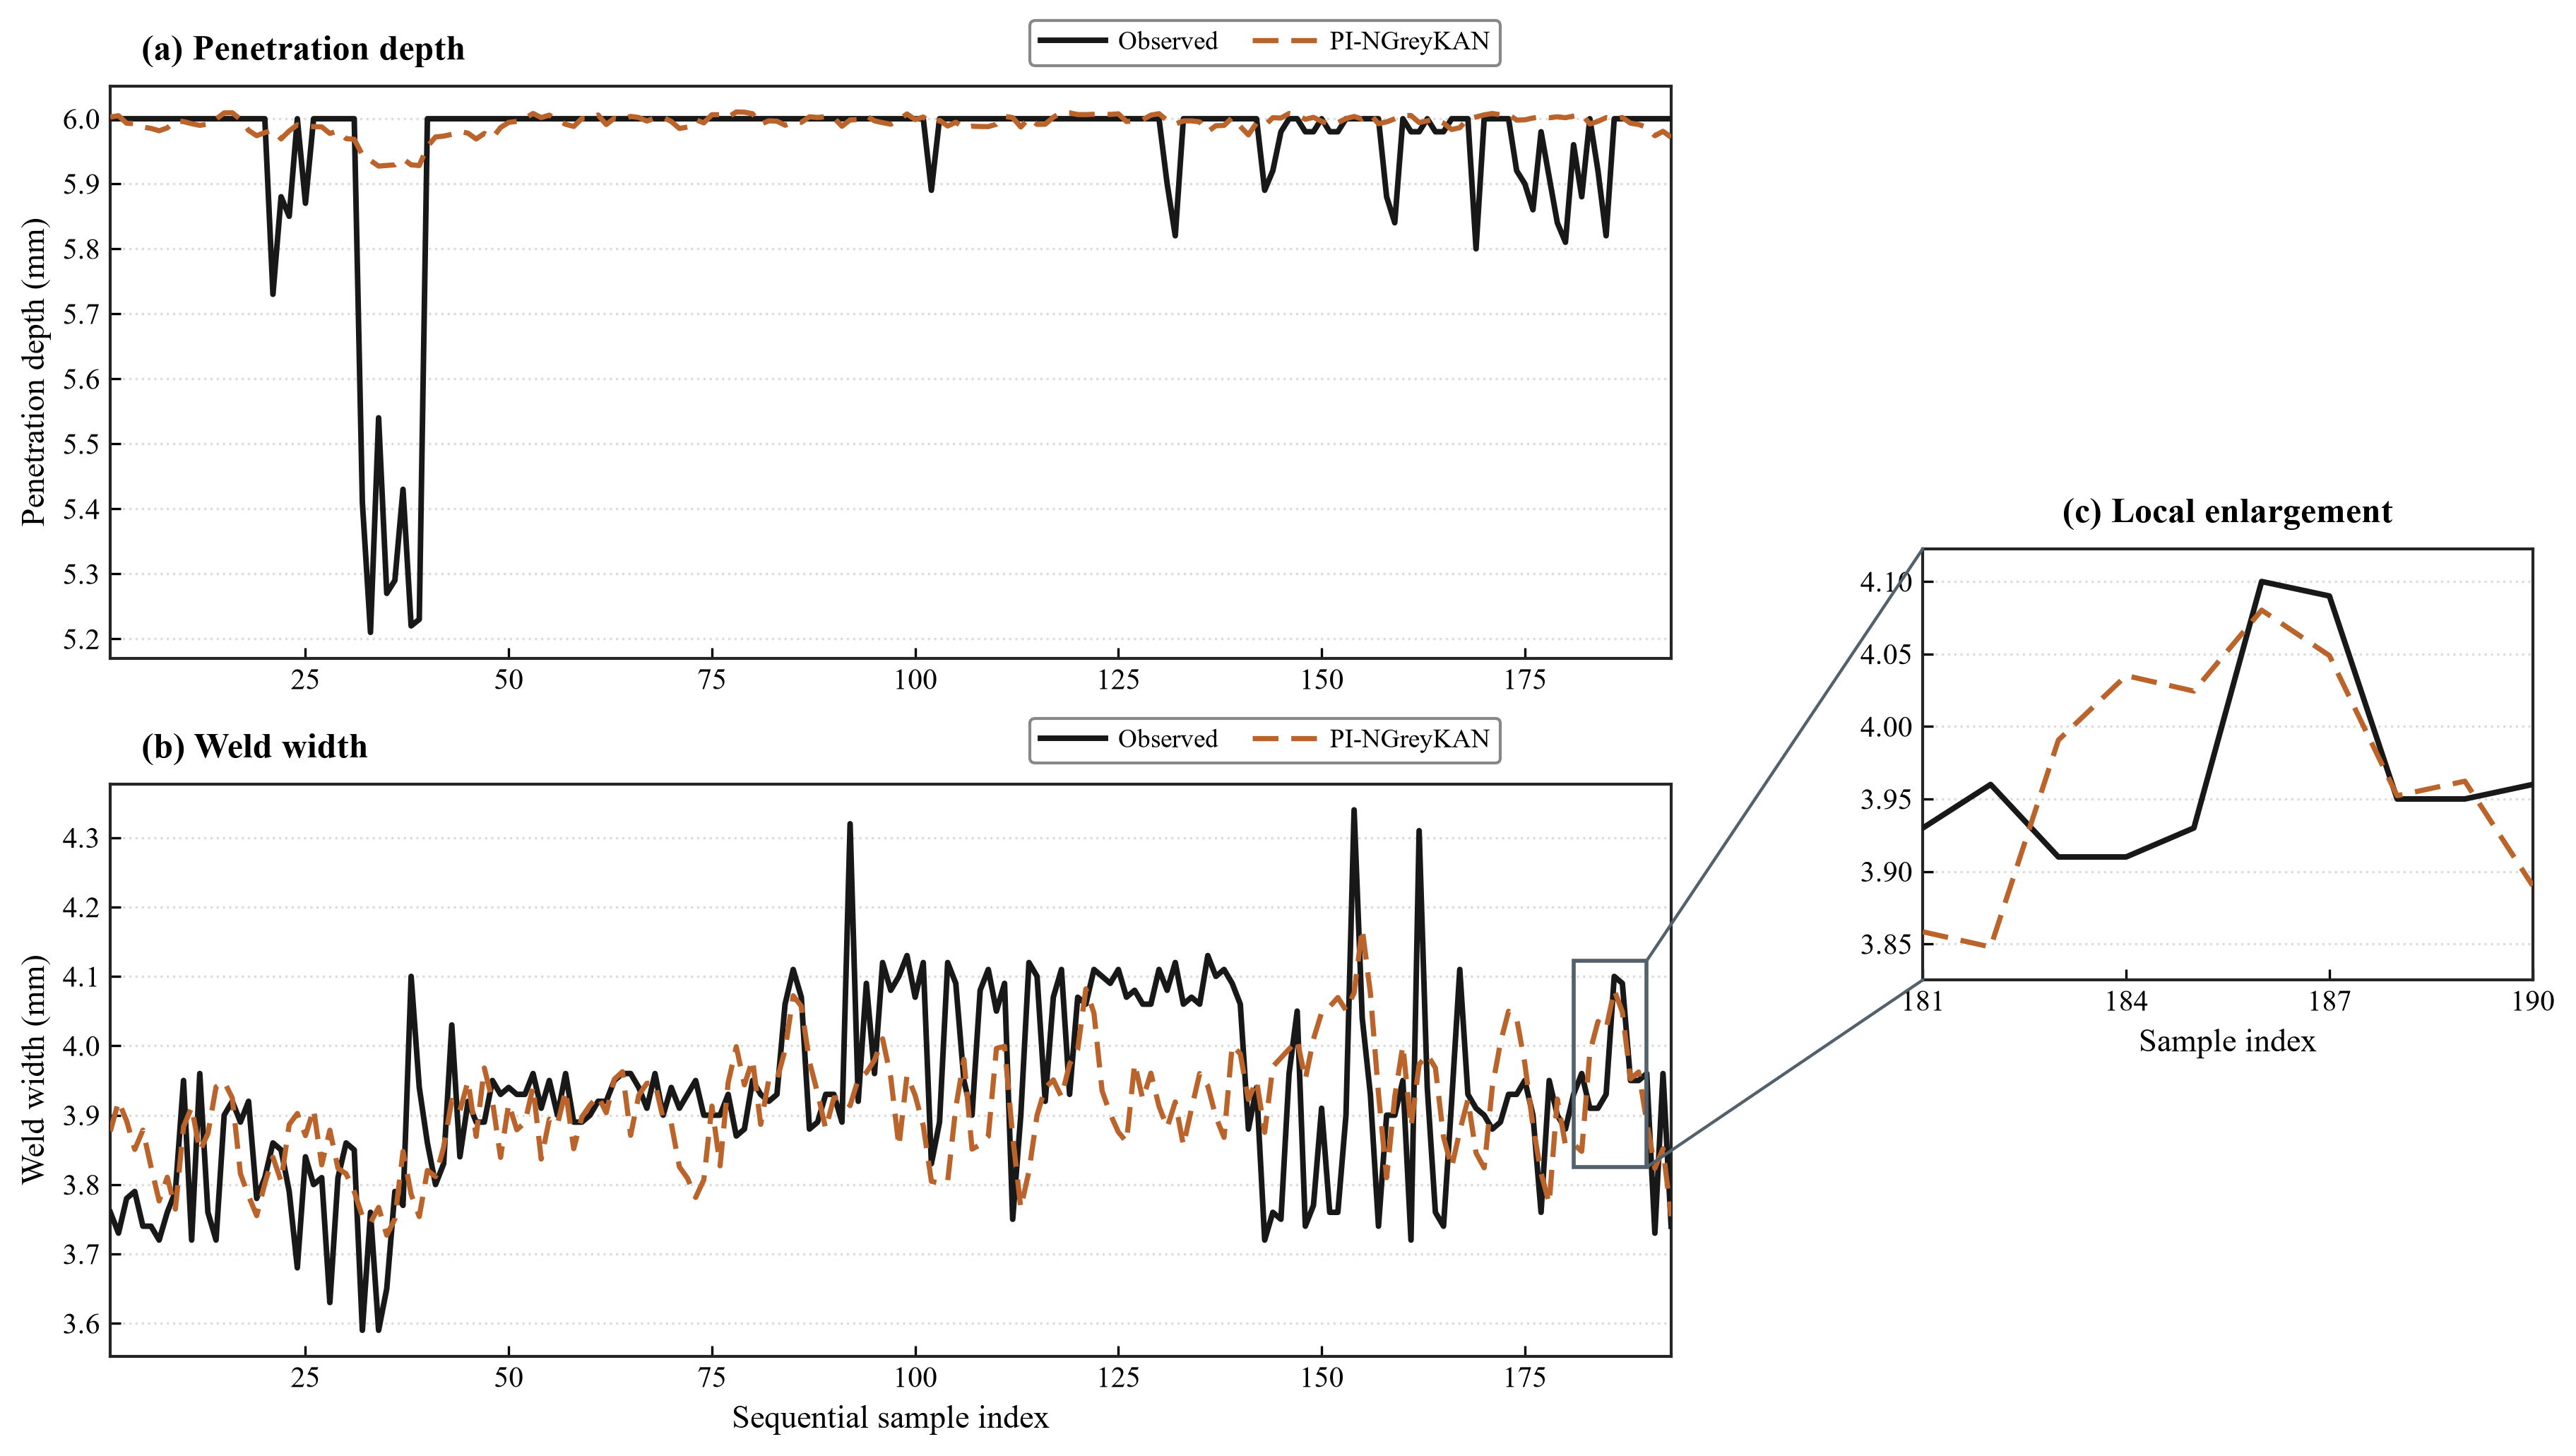
\includegraphics[width=0.92\linewidth]{figures/W09_Online_Replay_Depth_Width_300dpi.png}
    \caption{Independent sequential verification on Weld 09 using PI-NGreyKAN trained on all observations from Cases 1--4: (a) measured and predicted penetration depth; (b) measured and predicted weld width. W09 labels were not used in model training or inference.}
    \label{fig:w09_online_prediction}
\end{figure}

% ----- Inserted combined D/W error and tolerance table -----
\begin{table}[htbp]
    \centering
    \caption{External W09 prediction accuracy and error-tolerance coverage for weld penetration depth and width.}
    \label{tab:w09_online_metrics}
    \setlength{\tabcolsep}{5pt}
    \renewcommand{\arraystretch}{1.08}
    \begin{tabular}{lrr}
        \toprule
        Metric & Penetration depth & Weld width \\
        \midrule
        Number of observations & 193 & 193 \\
        MAE (mm) & 0.0478 & 0.0995 \\
        RMSE (mm) & 0.1345 & 0.1290 \\
        MAPE (\%) & 0.858 & 2.522 \\
        Mean bias (mm) & +0.0364 & -0.0195 \\
        MAE for $D=6$ mm (153 points) & 0.0089 & 0.0917 \\
        MAE for $D<6$ mm (40 points) & 0.1964 & 0.1294 \\
        Relative error $\leq 2\%$ (\%) & 90.2 & 49.7 \\
        Relative error $\leq 5\%$ (\%) & 95.9 & 85.5 \\
        Relative error $>5\%$ (\%) & 4.1 & 14.5 \\
        Relative error $>10\%$ (\%) & 2.6 & 0.0 \\
        Absolute error $\leq 0.1$ mm (\%) & 89.1 & 59.6 \\
        Absolute error $\leq 0.2$ mm (\%) & 94.8 & 85.5 \\
        \midrule
        Both targets within 5\% & \multicolumn{2}{c}{81.9\% (158/193)} \\
        \bottomrule
    \end{tabular}
    \par\vspace{3pt}
    \begin{minipage}{0.90\linewidth}\footnotesize
    \emph{Note:} This is an external, label-blind sequential replay of W09
    (193 observations) after fitting on all 528 observations of Cases 1--4.
    Results use the mean prediction from three independently fitted seeds.
    Percentages denote illustrative prediction-error tolerances, not industrial
    weld acceptance specifications. W09 labels are used only for post-hoc scoring.
    \end{minipage}
\end{table}

\subsection{Discussion and practical implications}
\label{sec:w09_discussion}

Although the overall penetration-depth MAPE is below 1\%, the W09 data contain a substantial concentration of observations at 6.00~mm: 153 of 193 observations (79.3\%). On these 153 observations, the complete model yields an MAE of 0.0089~mm, although this favorable value is partly attributable to the highly concentrated observed target distribution. However, its performance deteriorates for the remaining 40 observations with actual penetration depth below 6.00~mm, where MAE increases to 0.1964~mm and MAPE reaches 3.57\%. Notably, around observations 32--39, the measured penetration depth decreases to approximately 5.21--5.54~mm, while the model predictions remain close to 5.93--5.94~mm. The maximum absolute penetration-depth error is 0.7257~mm, highlighting a limitation in identifying abrupt, relatively rare under-penetration episodes.

To place these results in context, a constant baseline based on the median penetration depth of the training data (6.00~mm) was also evaluated without fitting to W09. This simple baseline yields a slightly lower penetration-depth MAE (0.0441~mm) than PI-NGreyKAN (0.0478~mm), although its RMSE is higher (0.1474~mm versus 0.1345~mm). Thus, the small overall MAPE alone does not establish superiority over a trivial predictor when the target distribution is strongly concentrated at its upper observed value. This result emphasizes the importance of examining both overall prediction errors and the subset corresponding to potentially safety-relevant penetration deficiencies.

For weld width, PI-NGreyKAN achieves a lower MAE (0.0995~mm) and RMSE (0.1290~mm) than the constant training-median baseline (0.0998~mm and 0.1323~mm). Nevertheless, only 85.5\% of predictions fall within a 5\% relative-error tolerance, compared with 91.2\% for the constant baseline. Accordingly, the evidence supports the feasibility of sequential dual-output inference, while indicating that prediction robustness is not uniformly improved under all performance criteria. An additional analysis of the input distributions indicates that a small number of W09 measurements extend beyond the ranges encountered in Cases 1--4, suggesting that cross-weld variation deserves attention in future evaluations.

A one-observation-at-a-time implementation of the same grey-state recursion was checked against full-sequence inference and produced numerically equivalent predictions (maximum absolute difference below $5\times10^{-7}$~mm). In the present CPU-based implementation, the median measured inference time was approximately 0.21~ms per observation for each trained model. These software measurements indicate low computational overhead; however, real-time performance on industrial control hardware and the practical reliability of abnormal-penetration warnings require further prospective validation. Future work should therefore prioritize broader multi-weld training data, additional examples of under-penetration, uncertainty-aware detection of abnormal events, and verification under actual online acquisition conditions.

\begin{figure}[htbp]
    \centering
    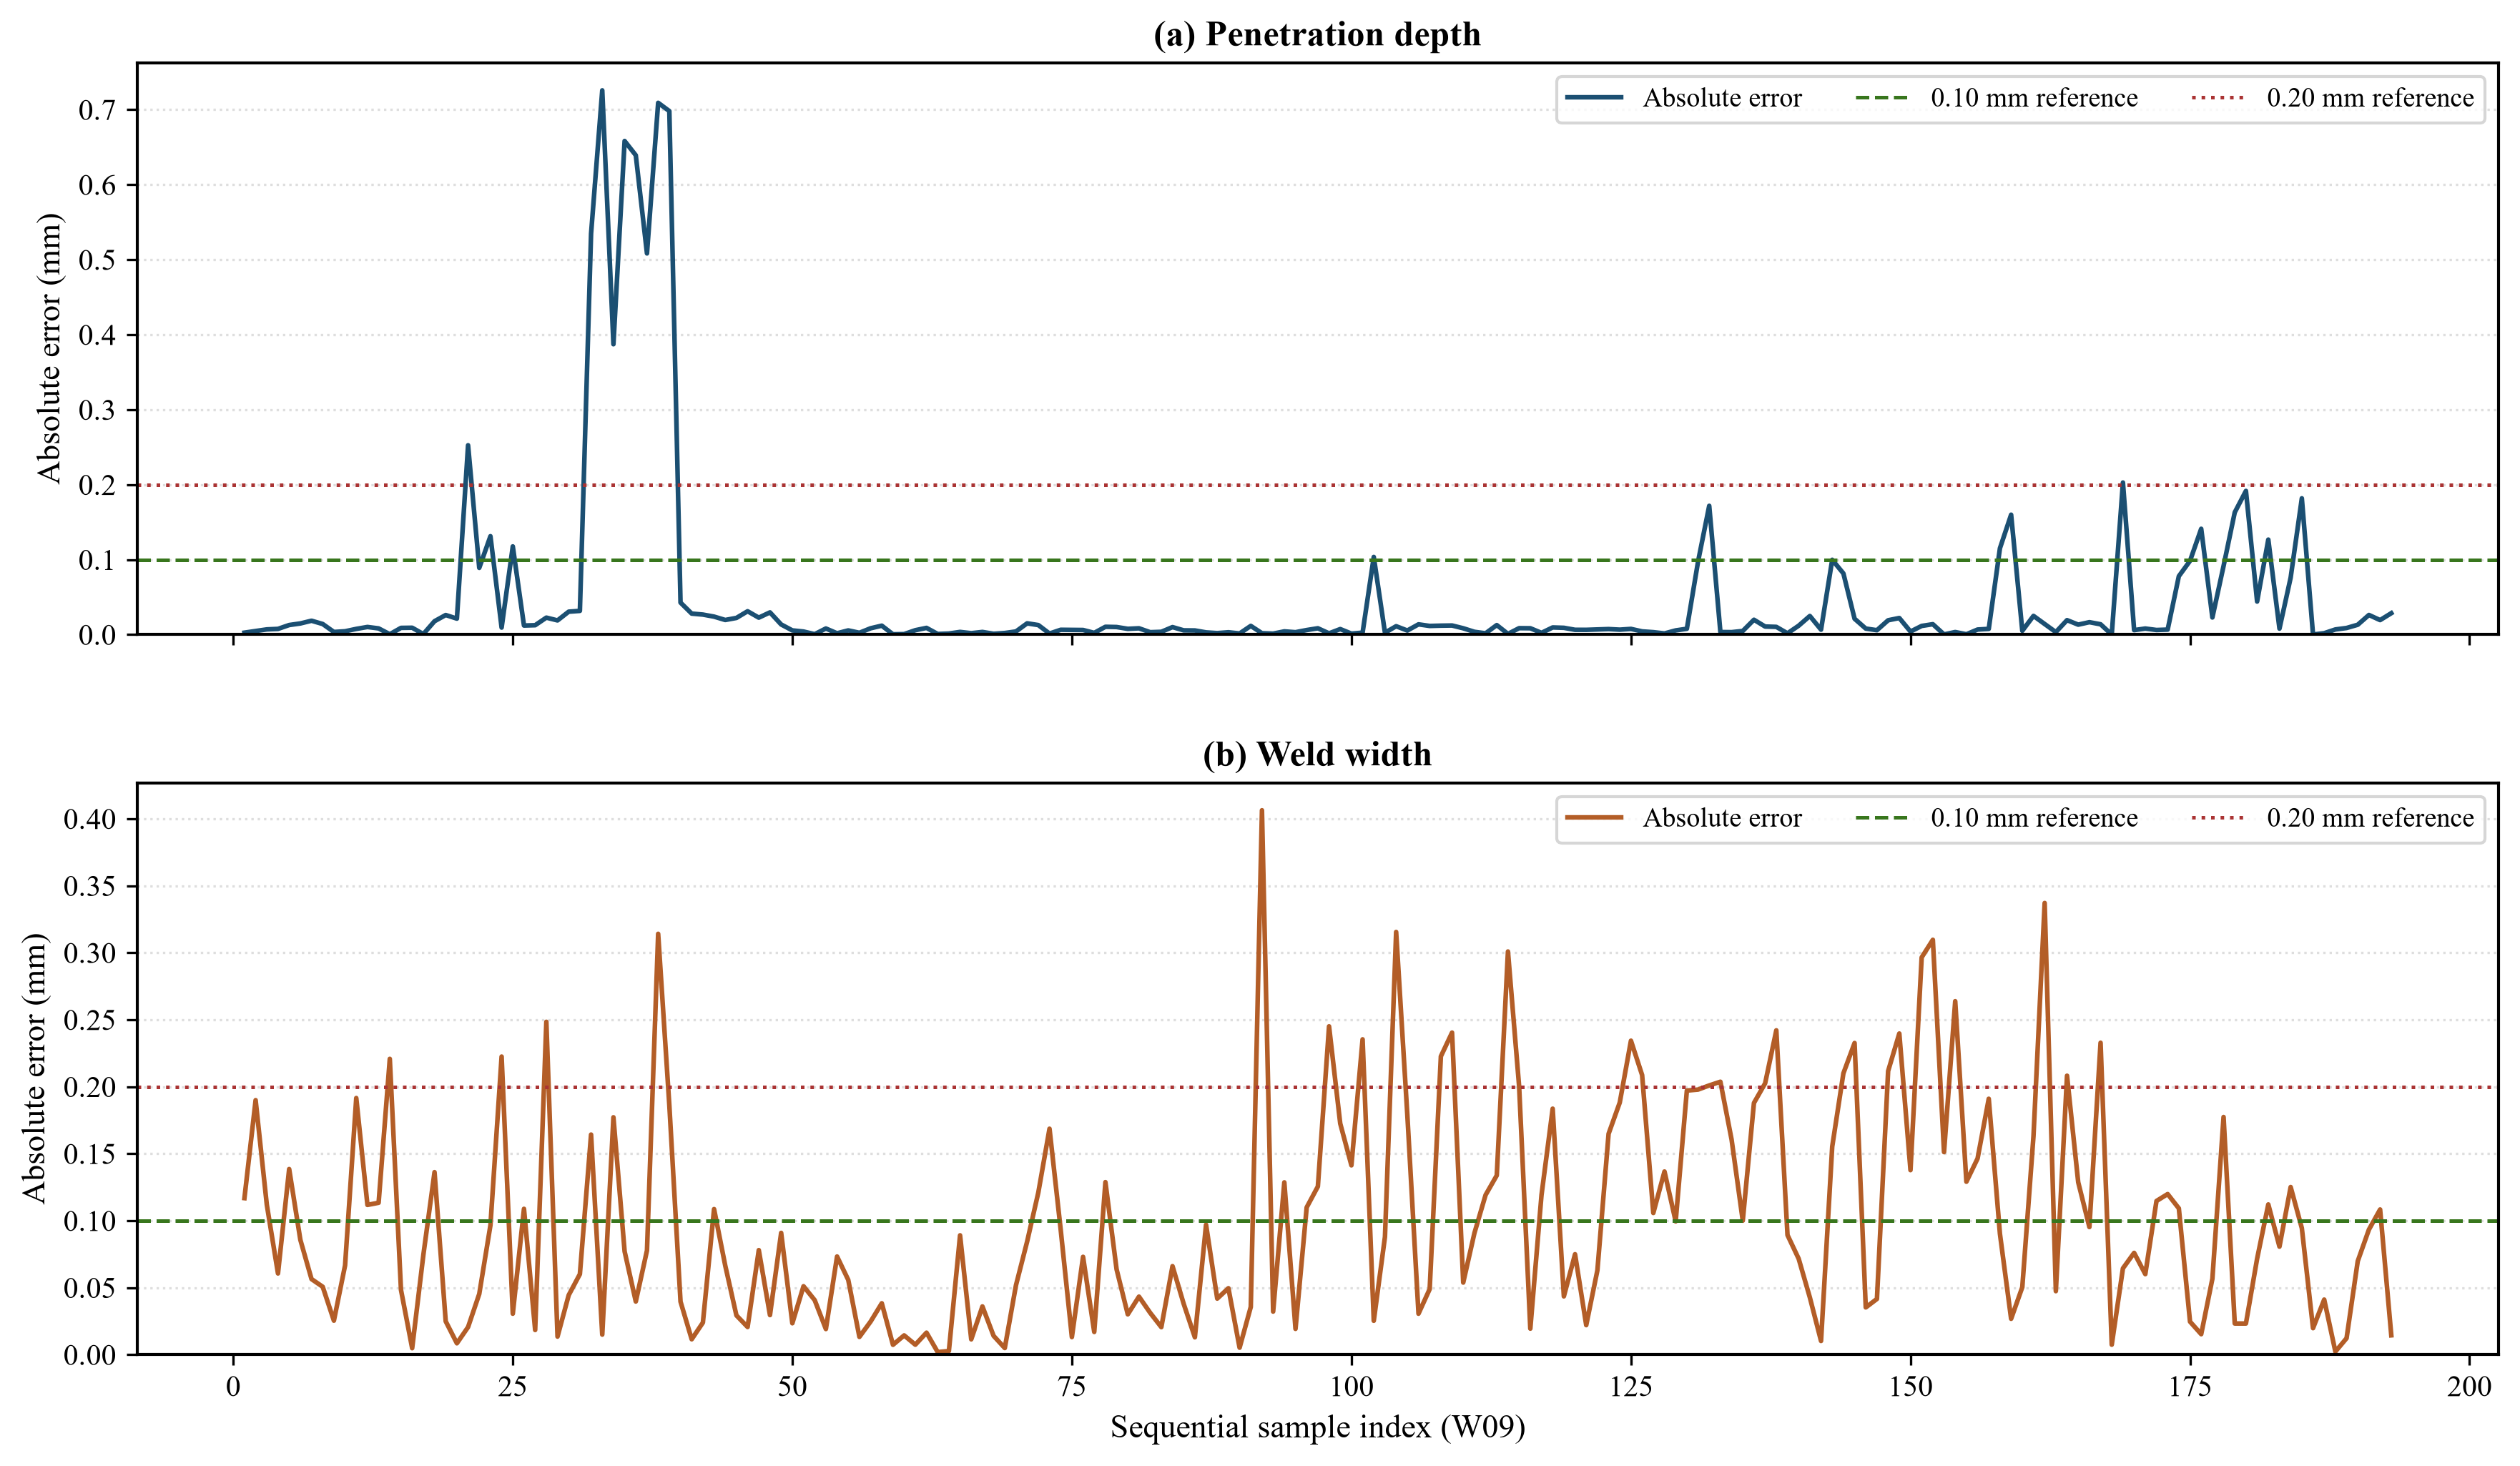
\includegraphics[width=0.92\linewidth]{figures/W09_Absolute_Errors_300dpi.png}
    \caption{Absolute prediction errors during independent sequential verification on Weld 09: (a) penetration depth; (b) weld width. Horizontal lines indicate illustrative absolute-error reference levels of 0.10 and 0.20~mm, rather than industrial acceptance specifications.}
    \label{fig:w09_absolute_errors}
\end{figure}
